\documentclass[12pt]{article}
\usepackage{setspace}
\usepackage{alltt}
\usepackage{tikz}
\usepackage{graphicx}
\usetikzlibrary{arrows}
\usepackage[margin=1in]{geometry}

\begin{document}

\doublespacing

\section{Phase I}
The software for Phase I responds to events from the timer and the buttons
using interrupts.

When a button is pressed, the event detects whether it is the first or second
button, or neither.
It sets a mode flag to either \texttt{LED} or \texttt{7SEG}, depending on which
button was pushed, and reads the current values from the switches to a stored
value.
Then, the value is displayed on the screen.
Finally, the timer period is restarted, and the count of periods elapsed is
reset to 0.

When a signal is received from the timer, the count of periods elapsed is incremented.
If this is the 9th period, the display is wiped, and the mode flag is set to \texttt{OFF}.
Otherwise, the $n$\textsuperscript{th} bit is displayed on the appropriate display.

Consider the following pseudocode.

\begin{alltt}
ON button INTERRUPT
    counter \(\gets\) 0
    value \(\gets\) led_pio_value
    mode \(\gets\) led IF button = 1 ELSE 7seg
    DISPLAY BIT counter OF value USING MODE mode
    RESET timer

ON timer INTERRUPT
    counter \(\gets\) counter + 1
    IF counter = 8
        mode \(\gets\) BLANK
    ELSE
        DISPLAY BIT counter OF value USING MODE mode
\end{alltt}

The behaviour of Phase I can also be modelled as a finite state machine, as in the
diagram below.

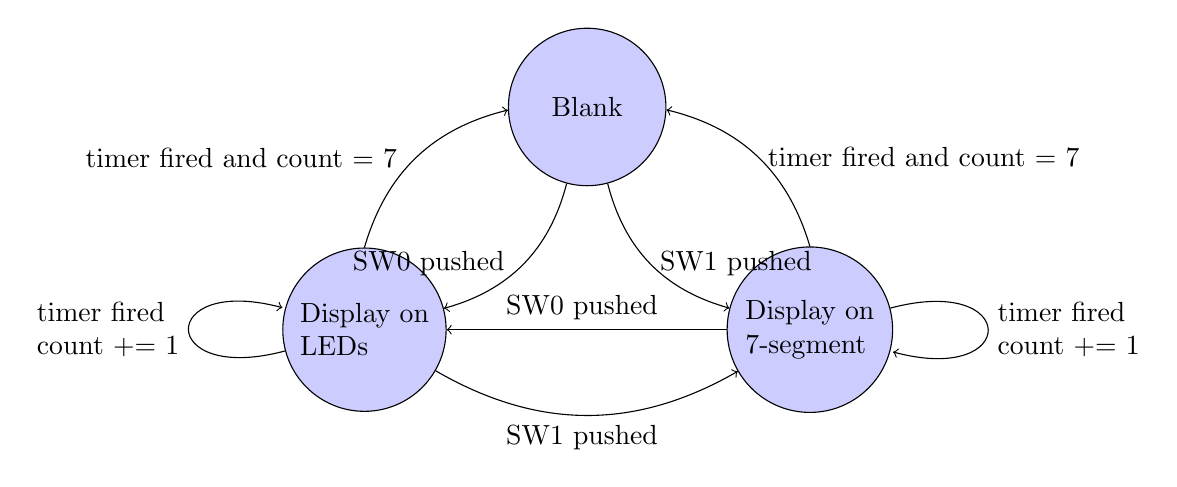
\begin{tikzpicture}[->,node distance=4cm,main/.style={circle,fill=blue!20,draw,minimum size=2cm,align=left}]
    \node[main] (blank) {Blank};
    \node[main] (led) [below left of=blank] {Display on\\LEDs};
    \node[main] (7seg) [below right of=blank] {Display on\\7-segment};
    \path[align=left]
        (blank) edge [bend left] node [left] { SW0 pushed } (led)
                edge [bend right] node [right] { SW1 pushed } (7seg)
        (led) edge [loop left] node { timer fired \\ count += 1} (led)
              edge [bend right] node [below] { SW1 pushed } (7seg)
        (led.north) edge [bend left] node [left] { timer fired and count = 7 } (blank)
        (7seg) edge [loop right] node { timer fired \\ count += 1 } (7seg)
               edge node [above] { SW0 pushed } (led)
        (7seg.north) edge [bend right] node [right] { timer fired and count = 7 } (blank)
    ;
\end{tikzpicture}

We initially used polling to detect button presses, and refactored the code
to use interrupts.
There is no discernable performance difference between the two techniques.
The initial technique used was tight polling, which was likely somewhat
faster than interrupt handling, because of the time taken for the context
switching.
However, any performance difference is likely on the range of microseconds,
and is totally insignificant compared to the time that it takes for the
user to push a button, or to perceive the change in display output.
Moreover, because there is no other background task to be run, it doesn't
matter how much CPU time is spent checking the state of the buttons or
timer.
This nullifies the primary disadvantage of tight polling.
However, writing the logic to be interrupt-driven makes the code more
understandable.
It eliminates the need for an event loop, since the response for each
action is triggered directly.
However, it does introduce boilerplate when setting up
and responding to interrupts.
This is more verbose than simply reading the value of the switch on repeat.

We took a manual approach to testing.
We would test the functionality of Phase I by loading the program onto the
board, then testing the response of the LEDs and 7-segment displays when
essentially arbitrary button presses were made.
During debugging, we would also have the program activate otherwise unused
LEDs to indicate that a particular section of code had been executed, or to
display the binary valuable of some variable of interest.
In particular, we displayed the binary pattern of the value being displayed
on the red LEDs.

One bug that we encountered was that the 9 bits from the switch input were
being displayed instead of 8, because of an off-by-one error in a comparison.
We noticed this after having written the second mode of the software to display
output on the 7-segment display.
Previously, this bug went undetected, because an extra 0 bit of output was
represented as the LED being off, which is indistinguishable from the cycle
being complete.
With the LED, the off state is distinct from the 0 state, so this bug was
fairly simple to detect with careful observation of how many outputs
were displayed.
The coding error itself was trivial to correct after it was noticed - it
simply meant stopping when \texttt{count = 7}, not \texttt{count = 8}
(bearing in mind that count begins at 0).

\newpage
\section{Phase II}
The two different synchronization techniques were written using different
functions, each one setting up any state it needed, and tearing down any
state it had mutated when it was done. This allowed us to easily switch
between the two techniques when testing, and allowed us to create our
measured results very quickly as well.

\subsection{Occasional Polling}
Our approach for the occasional polling technique was very simple, effectively
just the busy-loop approach, but with the addition of doing work \emph{inside}
the busy-loop, allowing us gain some efficiency, at the cost of increased
latency proportional to the grain size given. Note that the inner loop used
to create the following charts was the grain size, which caused some pretty
significant ossicalations for the occasional polling solution.

\begin{alltt}
state \(\gets\) LOW
LOOP 200 TIMES
    WHILE pulse flag has not changed
        run background task with grain size
    state \(\gets\) !state
    respond to the pulse with state
\end{alltt}
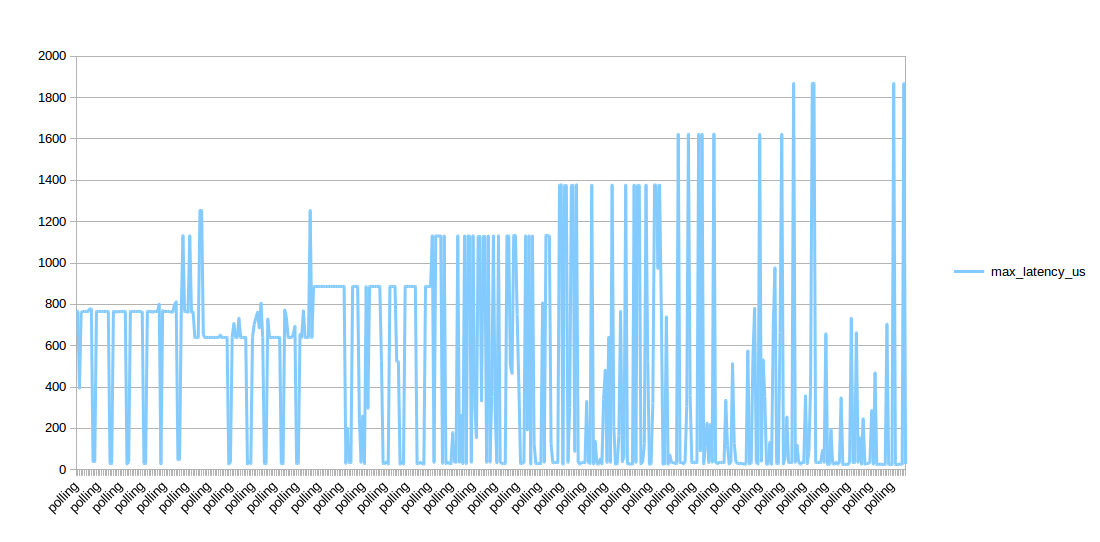
\includegraphics[width=\textwidth]{polling_max_latency.png}
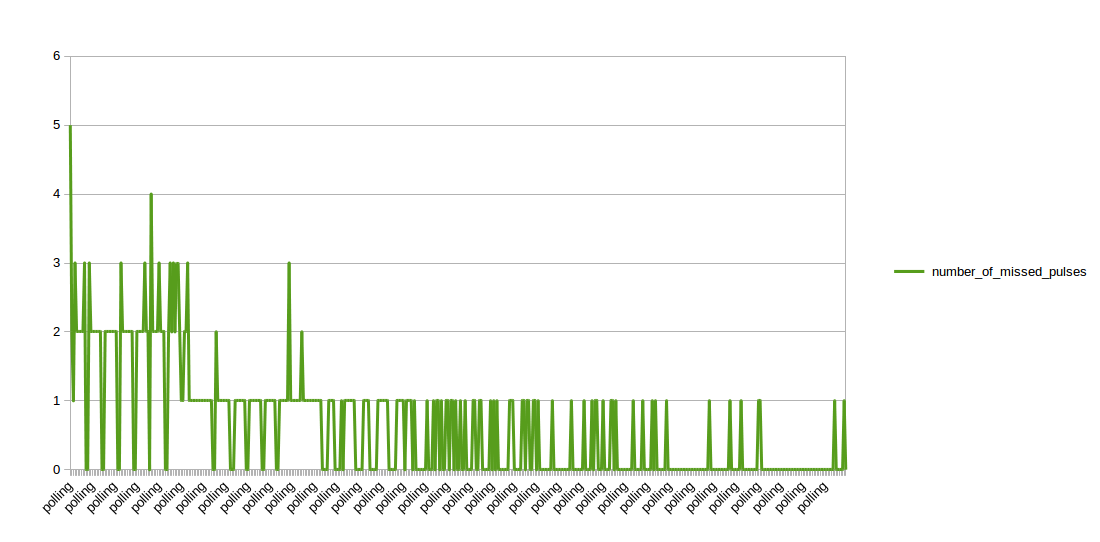
\includegraphics[width=\textwidth]{polling_missed_pulses.png}
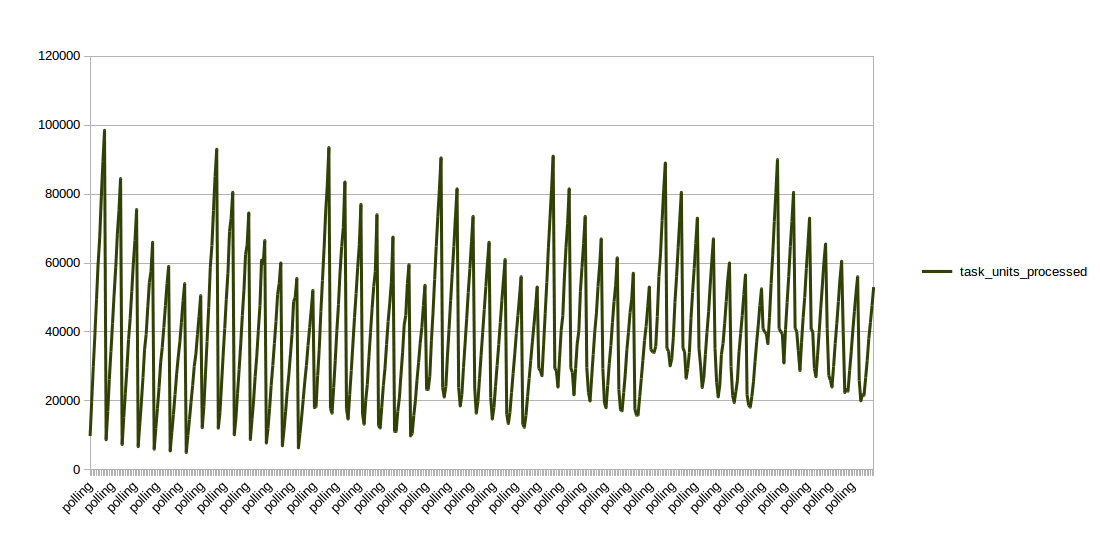
\includegraphics[width=\textwidth]{polling_units_processed.png}

\subsection{Interrupts}
For our interrupt-based approach, we ran the background task directly, in what
appears to be a never-ending loop. However, interrupts will interrupt this
endless loop, respond to the EGM immediately, and update the pulse\_count
variable which the main thread uses to eventually exit. This approach had very
low latency and predictable performance, regardless of parameters provided.

\begin{alltt}
pulse_count \(\gets\) 0
while pulse_count < 200
    run background task with grain size

ON pulse INTERRUPT
    state \(\gets\) current level
    reset the pulse edge capture register
    respond to the pulse with state
    pulse_count \(\gets\) pulse_count + 1
\end{alltt}

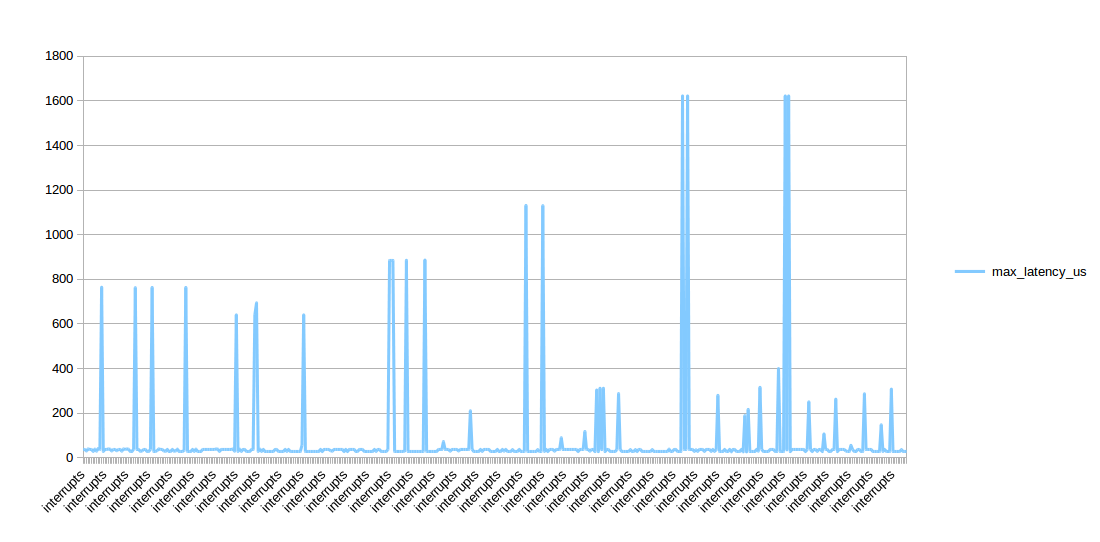
\includegraphics[width=\textwidth]{interrupts_max_latency.png}
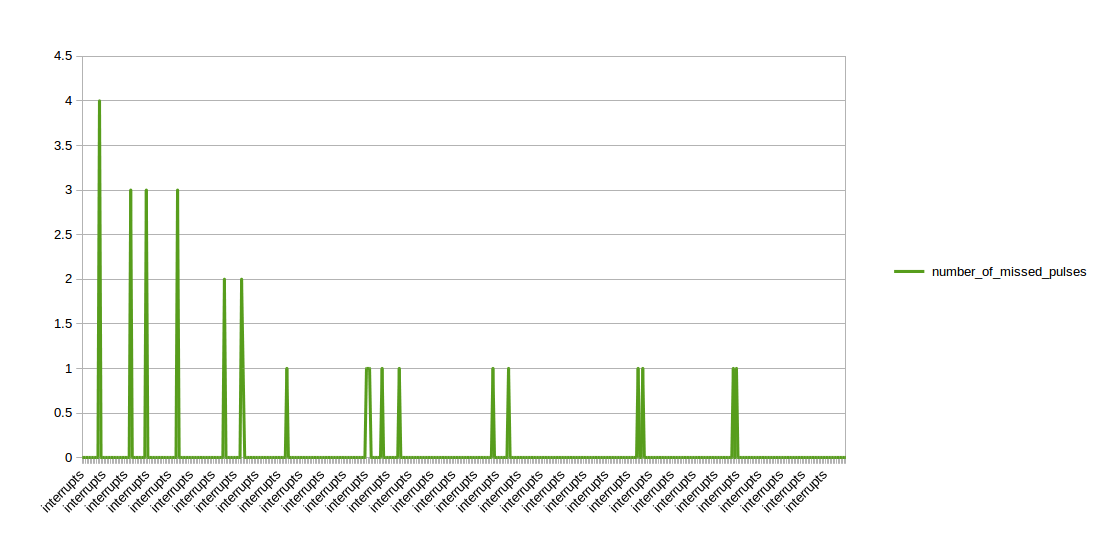
\includegraphics[width=\textwidth]{interrupts_missed_pulses.png}
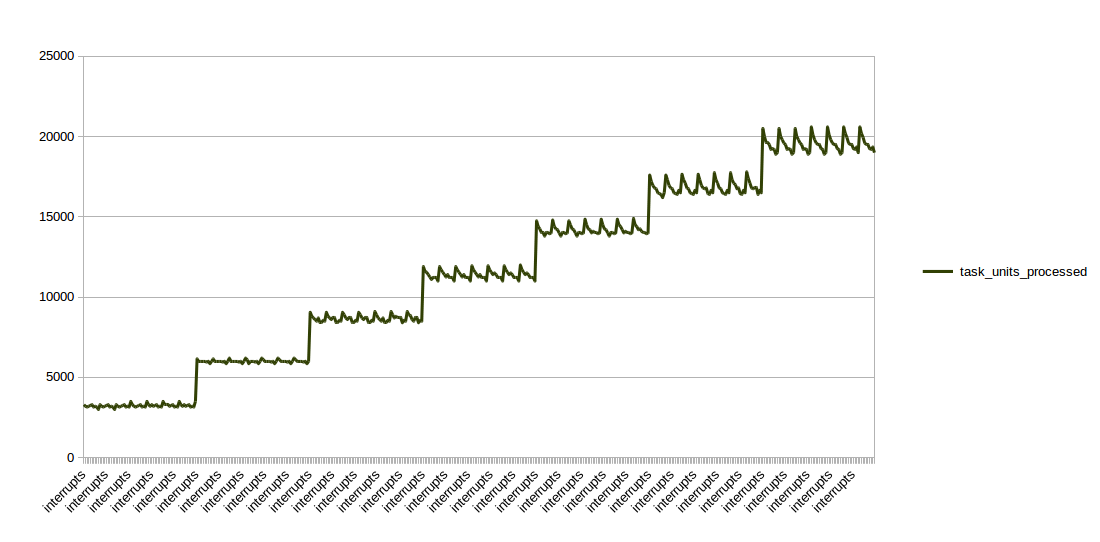
\includegraphics[width=\textwidth]{interrupts_units_processed.png}

\newpage
\section{Contribution and Reflection}
Peter Raboud:

I was responsible for writing up the part of the lab report pertaining to Phase I.
Justin and I equally shared the responsibility for writing the software itself.
The most important thing I learned during this lab is how to effectively write
software with interrupts.
I have written interrupt handlers before as part of CS 350, to handle memory
faults, etc.
However, these operated solely on kernel data structures, and don't typically
interact with user-level programs.
The way that we used interrupts, in Phase I in particular, meshed user code and
interrupt handler code far more than I had done in the past.
The resulting code used interrupts as the primary form of control flow, with
very little logic being handled synchronously.
This was useful practice for writing event-driven programs.

Justin McGirr:

I was responsible for writing the part of this lab report pertaining to Phase II.
Peter and I equally shared the responsibility for writing the actually software
of the lab. The most useful things I learned were that Nios is flacky, and
will break if you aren't careful with it, as well as re-iterating why interrupts
are most typically used for listening for events (as opposed to any kind of
polling).
\end{document}
